\documentclass[../Main.tex]{subfiles}
\begin{document}
\newpage
\section{Database}
\subsection{Database structure}
For our database we use Cassandra \cite{cassandra}. Cassandra makes use of a structure where the top level of your data are keyspaces. This means all data tables are distributed throughout keyspaces. You can specify the distribution per keyspace. A keyspace then contains different tables. \\

Each table has a partition key which is used for the distribution, since a single partition is always on a single server. In the tables below, we will refer to a partition key by ‘K'. The rest of the primary key is defined with clustering keys, which have a sorting order. We will refer to a clustering key by ‘C'. The sorting order is indicated by means of an arrow. More specifically, an arrow pointing up, $\uparrow$, is used to indicate a column in a table that is sorted in ascending order (i.e., from lowest (in the topmost row) to highest (in the bottom-most row)). Similarly, an arrow pointing down, $\downarrow$, next to a column is used to indicate that the table is sorted on the column in descending order.\\

The structure of our database consists of two keyspaces. One keyspace for the data about the jobs and one with all the data about the methods and projects in the database. 

\subsubsection{Jobs}
The keyspace with the jobdata, called \texttt{jobs}, contains the following table:

\begin{table}[h]
    \centering
    \begin{tabular}{|ccc|}
\hline
    \multicolumn{3}{|c|}{\textbf{jobsqueue}}   \\
    \hline
    Constant & Int & K \\
    Priority & Bigint & C\,$\uparrow$ \\
    Jobid & UUID & C\,$\downarrow$ \\
    Url & Text & \\
    \hline
\end{tabular}
\end{table}

As we can see, the jobs queue is sorted with ascending order on the \texttt{Priority} and descending on the \texttt{Jobid}. The \texttt{Constant} is included to make sure that the whole \texttt{Jobqueue} is part of a single partition and can therefore be sorted on the priority. The priority is a 64-bit integer which is calculated as the current time minus the priority score we get from the crawler. The priority is sorted from lowest to highest so the job with the lowest priority will be done first. The job id is a Universally Unique Identifier (or UUID) so it becomes easier to keep track of the different jobs. Finally, the \texttt{Url} is the url that should be parsed when this job is done.

\subsubsection{Projectdata}
The other keyspace, called \texttt{projectdata}, contains the data for the methods and projects that we store. The first table is the table containing the methods:

\begin{table}[h]
    \centering
    \begin{tabular}{|ccc|}
\hline
    \multicolumn{3}{|c|}{\textbf{methods}}   \\
    \hline
    Method\_hash & UUID & K \\
    ProjectID & Bigint & C\,$\uparrow$\\
    StartVersionTime & Timestamp & C\,$\downarrow$\\
    File & Text & C\,$\downarrow$\\
    StartVersionHash & Text & \\
    EndVersionTime & TimeStamp & \\
    EndVersionHash & Text & \\
    Name & Text & \\
    LineNumber & Int & \\ 
    Authors & \{UUID\} & \\
    Parserversion & Bigint & \\
    \hline
\end{tabular}
\end{table}

Here the \texttt{Method\_hash} is the hash of the method obtained by the parser. The \texttt{ProjectID} is the identifier of the repository this method was found in. The \texttt{StartVersionTime} is the timestamp of commit that is the first version this method was found in. The \texttt{File} is the name of the file this method was found in including the path of the file. The \texttt{StartVersionHash} is the hash of the commit from the first version of this method. The \texttt{EndVersionTime} and \texttt{EndVersionHash} are respectively the timestamp and the hash of the commit for the latest version this method was found in. The \texttt{Name} is the name of the method and the \texttt{LineNumber} is the number of the line this method starts in the file. The \texttt{Authors} is a set of UUIDs for the authors that have worked on this method. Finally the \texttt{Parserversion} is the version of the parser used to parse this method.\\

The next table is for the data about the projects:

\begin{table}[h]
    \centering
\begin{tabular}{|ccc|}
    \hline
    \multicolumn{3}{|c|}{\textbf{projects}} \\ \hline
    ProjectID & Bigint & K \\
    VersionTime & Timestamp & C\,$\downarrow$ \\
    VersionHash & Text & \\
    License & Text & \\
    Name & Text & \\ 
    URL & Text & \\
    OwnerID & UUID & \\
    Hashes & \{UUID\} & \\
    Parserversion & bigint & \\
    \hline
\end{tabular}
\end{table}

In this table the \texttt{ProjectID} is the identifier for the repository. The \texttt{VersionTime} and \texttt{VersionHash} are respectively the timestamp and hash of the commit for this version of the project. The \texttt{License} is the license of the project retrieved from git. The \texttt{Name} is the name of the project. The \texttt{URL} is the url where the project can be found. The \texttt{OwnerID} is the UUID for the owner of the project. The \texttt{Hashes} is a set of hashes of the methods in this project. Finally the \texttt{Parserversion} is the version of the parser used to parse this project.\\

Since Cassandra is a non-relational database, a relation between a method and its authors is not directly available. A new table, \texttt{method\_by\_author}, has to be introduced to relate the authors to methods. More precisely, the following table is used to find the methods created by a certain author:

\begin{table}[h]
    \centering
\begin{tabular}{|ccc|}
\hline
    \multicolumn{3}{|c|}{\textbf{method\_by\_author}}   \\
    \hline
    AuthorID & UUID & K \\
    Hash & Text & C\,$\uparrow$\\
    ProjectID & Bigint & C\,$\uparrow$\\
    StartVersionTime & Timestamp & C\,$\downarrow$\\
    File & Text & C\,$\uparrow$\\
    \hline
\end{tabular}
\end{table}

Here the \texttt{AuthorID} is the ID of the author. The \texttt{Hash} is the hash of the method. The \texttt{ProjectID}, \texttt{StartVersionTime} and \texttt{File} correspond to the other parts of the primary key for the methods table.\\

Finally we have the table containing the authors:

\begin{table}[h]
\centering
\begin{tabular}{|ccc|}
\hline
    \multicolumn{3}{|c|}{\textbf{author\_by\_id}}   \\
    \hline
    AuthorID & UUID & K \\
    Name & Text & \\
    Mail & Text & \\
    \hline
\end{tabular}
\end{table}

In this table the \texttt{AuthorID} is the id of the author which is determined by hashing the name and mail. The \texttt{Name} and \texttt{Mail} are respectively the name and mail of the author.

\subsection{Distributed database}
\newpar{Distributing with Apache Cassandra}
For the distribution of the database we used an existing database system: Apache Cassandra \cite{cassandra}. Apache Cassandra automatically distributes the data in the database over the database servers connected to the network, we will refer to these servers as nodes from here on out. Cassandra has an ingenious internal system to correctly distribute the data over the connected nodes. We can specify how many copies of each piece of data should be stored in the database. In Cassandra we specified each server as a datacenter, this means that we can even specify how many copies of each piece of data should be stored on each server. We currently have three servers on which data is stored, when we hand over the project the system will keep running on two of those servers. In our current settings we have set the number of copies of each piece of data that should be stored in the database to two, this can be changed at any time. Also, Cassandra automatically stores these copies on different nodes, so every piece of data is stored on two different database nodes. When we upload data to the database, Cassandra will automatically store it on a node and store duplicates of all the data on a different node. 

\subsubsection{Node failure}
When Cassandra notices that a database node has gone down, it will automatically try to redistribute the data over the rest of the nodes. We also have a dashboard which shows if a database is up or not. When a node goes down, the maintainer is able to see this in this dashboard. The maintainer can then restart the node and when Cassandra notices that the node has reconnected it will once again redistribute the existing data. 

\subsubsection{Data redundancy}
As mentioned before, with the current Cassandra settings every piece of data is stored in the database on two different nodes. This means that one node can go down without any data loss. After the node goes down, Cassandra will redistribute the data, so now there are once again two copies of each piece of data. As a result, it is again made possible for a node to go down without any data loss. \\

It should be mentioned, however, that when all nodes are down, all data will be lost. Also, when two nodes go down in such quick succession that Cassandra does not have time to redistribute the data, we may also suffer data loss. This latter risk can be reduced by storing more than two copies of each piece of data, which is not hard to set up. 

\subsection{Maintainer dashboard}
We also have a website with information about the database displayed in graphs. Information we display here is real-time and is about disk usage per server, number of partitions per table in the database and disk usage per table. This website is designed for maintainers and can only be accessed with a username and password. These should only be known by maintainers of the system or people trusted by the maintainers who need this information for research purposes, for example. A screenshot can be seen in \cref{fig:dashboard}.
\begin{figure}
    \centering
    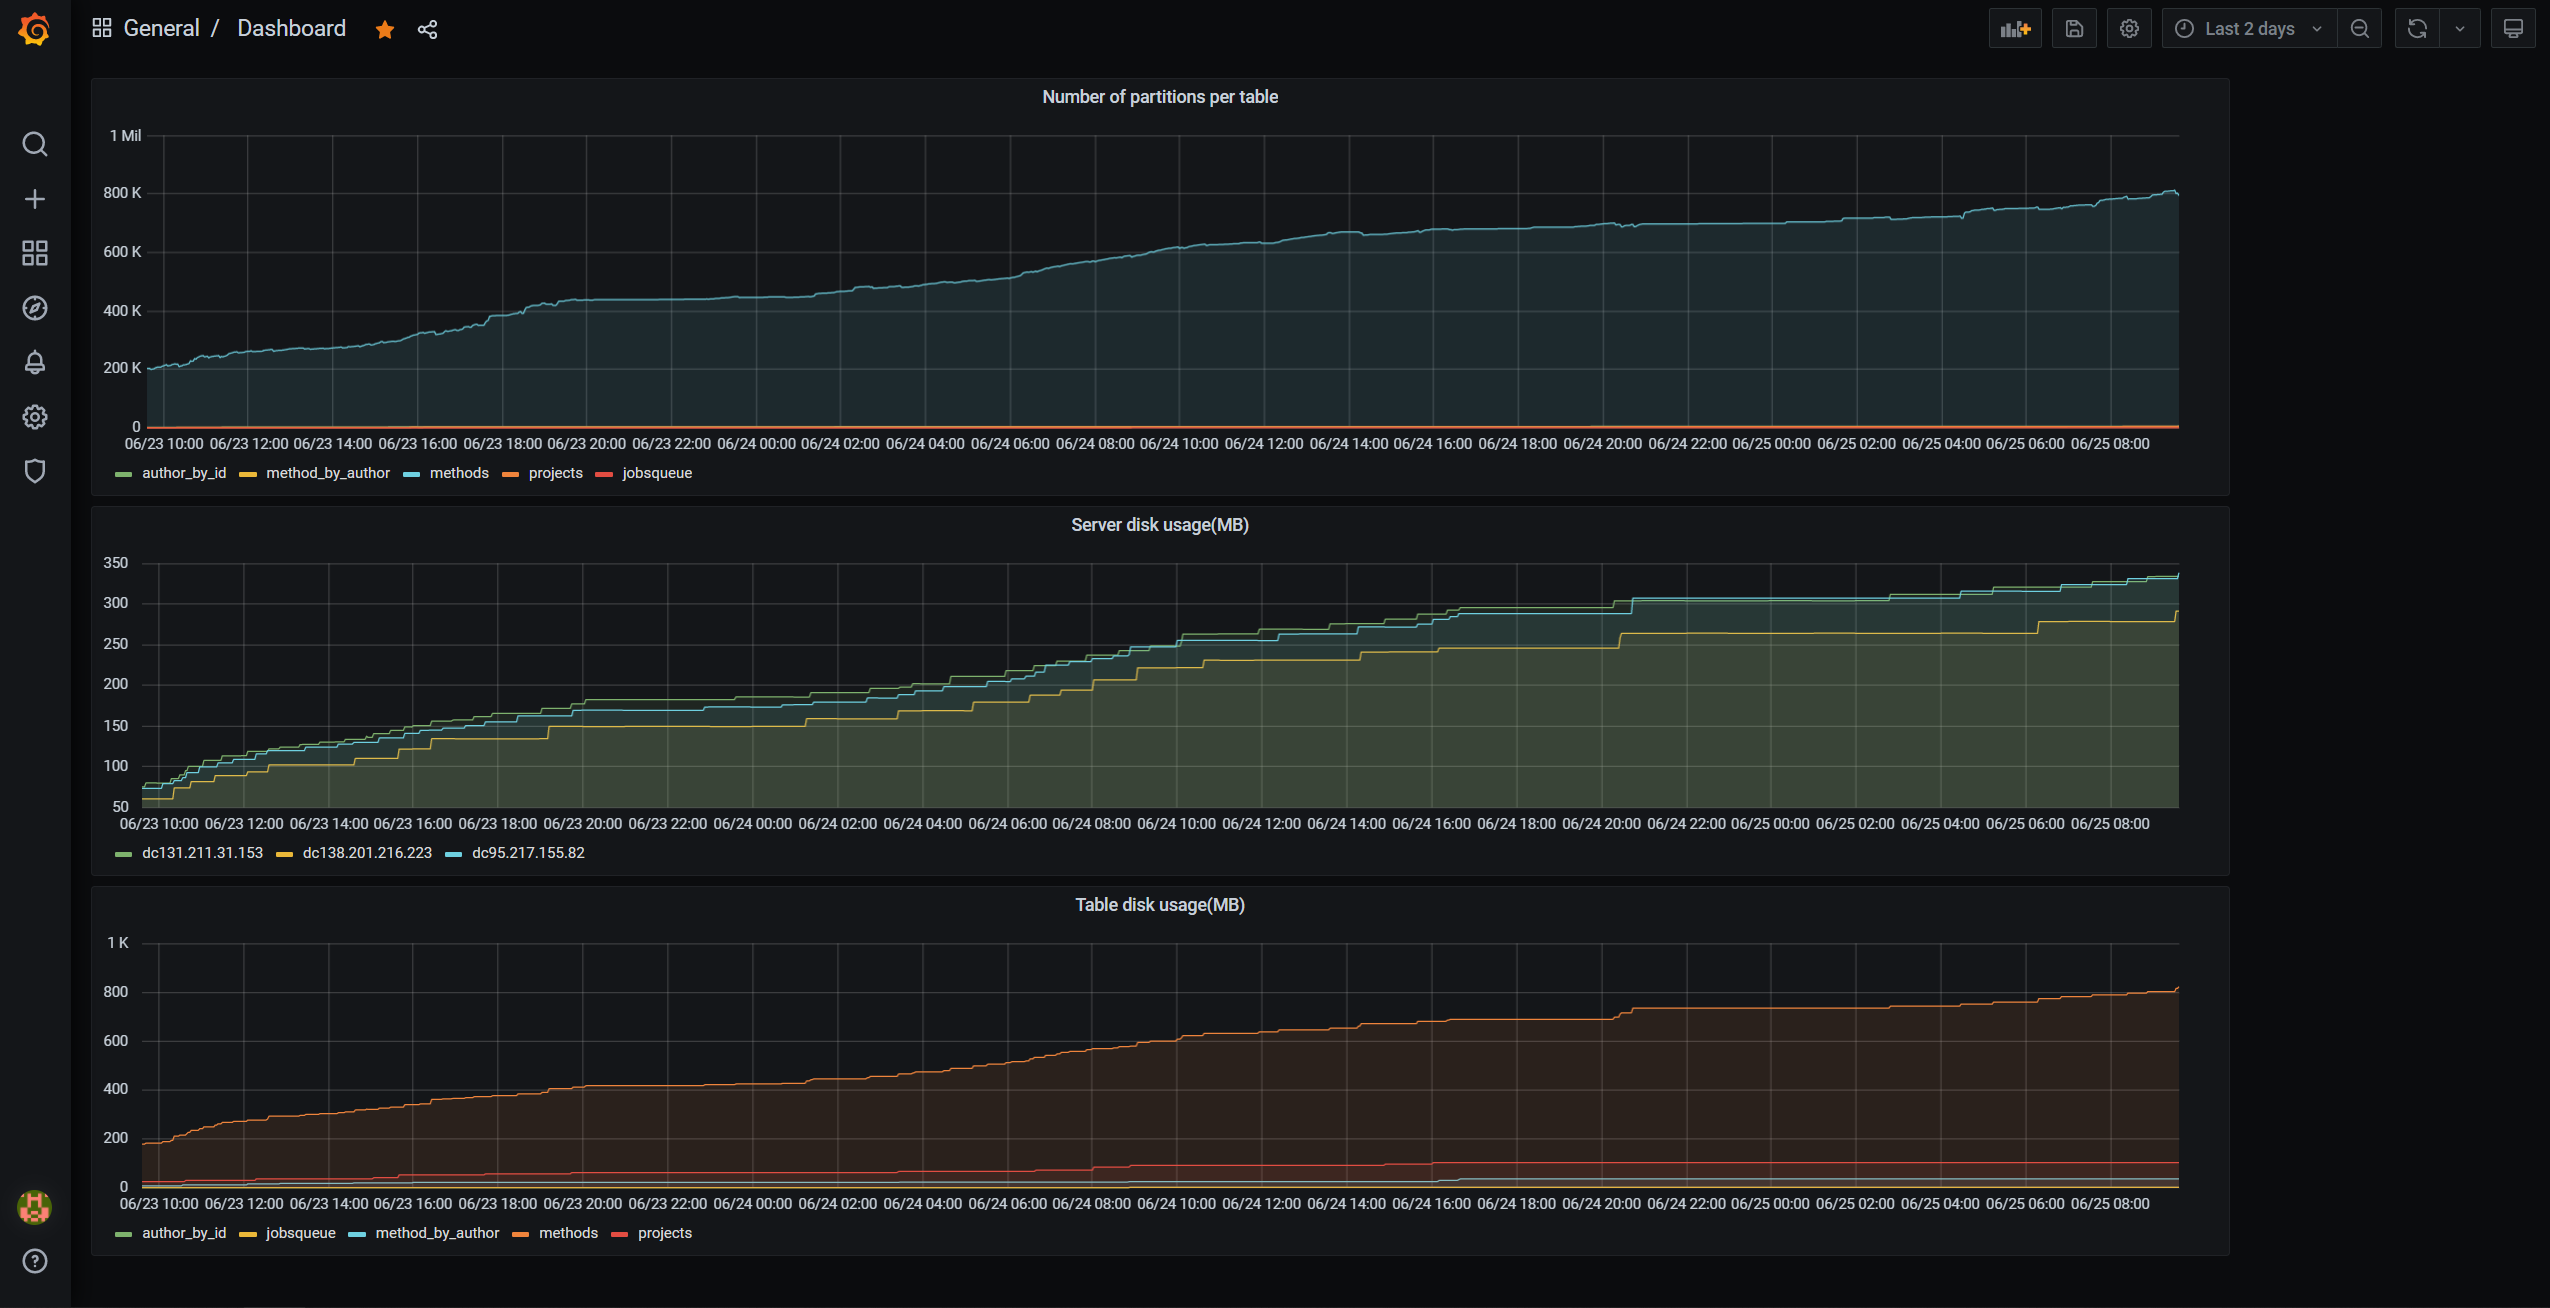
\includegraphics[width=\textwidth]{Dashboard.png}
    \caption{A screenshot of the maintainer dashboard}
    \label{fig:dashboard}
\end{figure}

\subsubsection{How it works}
The dashboard first uses \href{https://github.com/instaclustr/cassandra-exporter}{cassandra-exporter} to show the statistics to other programs. Next we use \href{https://prometheus.io/}{Prometheus} to collect the data. Finally we use \href{https://grafana.com/}{Grafana} to nicely visualise the statistics and host the website.

\section{Database API}
The Database API is responsible for multiple tasks. It handles the requests from the Controller to add data to the database and retrieve information about this data from the database. It is also responsible for the job distribution, for which it will give jobs to the worker nodes that ask for it. The class structure can be seen in \cref{fig:umldatabase}.\\

The \texttt{Database-API} class is the entrypoint for the program. The \texttt{ConnectionHandler} is responsible for handling the requests from the Controller, other servers or other clients. It will listen for requests on a specified port and retrieve the given data. It then passes this data to the \texttt{RequestHandler}, which parses the request to know what has to be done. If it is a request directed to the data in the database it is passed to the \texttt{DatabaseRequestHandler}. If the request is for the job distribution the request is passed to the \texttt{JobRequestHandler}. The \texttt{DatabaseConnection} and \texttt{DatabaseHandler} are responsible for the connection with the database and the \texttt{RAFTConsensus} is responsible for the implementation of the RAFT system, which will be explained in more detail later.

\subsection{Database Handling}
For requests that have something to do with the data corresponding to the methods in the database there is a method called in the \texttt{DatabaseRequestHandler} from the general \texttt{RequestHandler}. In most cases this method will first parse the input by splitting the input and if necessary parsing it to the correct objects. After this multiple threads are started and a queue is created. Each thread will take an element from the queue and pass this to method in the \texttt{DatabaseHandler} which will actually perform the database queries. After all queries are completed the threads are stopped and the result is parsed to the resulting string which is then returned.\\

The possible request are:
\begin{itemize}
    \item Upload project: Will upload all data for a project to the database. This includes the metadata of the project and all methods in the project. Optionally, a project can be updated based on a previous version of a project (which should already be in the database, of course). This is done by providing the previous version of the project together with a list of unchanged files. The methods in these unchanged files are then updated accordingly by updating their end version, and other, non-key, attributes.
    \item Check methods: Will take in a list of hashes and match these against the hashes in the database. It will then return all matches found in the database.
    \item CheckUpload project: Will perform both previous request by both adding the project to the database and match the methods in this project to the methods in the database.
    \item Extract project: Returns the metadata corresponding to a project.
    \item Get author: Retrieves the author corresponding to the passed ID.
    \item Get method by author: Returns the methods know to be worked on by the given author.
\end{itemize}

\subsection{Job distribution}
The Job queue itself is part of the Database, and is hence also distributed. However, for the Job queue we wanted to go a step further and make sure we are not handing out the same job multiple times. To accomplish this, we implemented a RAFT Consensus system.\\

In a RAFT system\footnote{\url{https://raft.github.io/}},
there is one leader node. The rest of the nodes are all non leader nodes. Once in a while, the leader node sends a heartbeat to all other nodes in the network. This heartbeat contains any information that needs to be synced between the nodes. The other benefit of this heartbeat is that we know for sure the leader is still running if we get one. Non-leader nodes do only one thing, and that is passing request on to the leader node. The leader node is the only node that actually executes the requests.\\ 

In this system, there is no problem when a non-leader node drops out. However, if the leader node drops out it becomes a bit harder. In our system, we made sure to sync the list of non leader nodes between all nodes in the network using the heartbeat. We make sure that the list is in the same order on all nodes. When the non leader nodes detect that the leader has dropped out, the new leader will be chosen. The new leader will always be the next node in the list of non leader nodes.\\\\
The Job request handler is the class that will actually handle the incoming requests for the Job queue. These requests include:
\begin{itemize}
    \item Get top job: Returns the next job in the job queue. If the job queue is under a specified threshold (which can be edited in \texttt{JobRequestHandler.h}), it will return a crawl job to refill the job queue. It will not return a crawl job if there is currently another worker node crawling. A crawl job will also be returned if the previous crawl job has not returned jet and has taken longer than a specified timeout time (which also can be edited in \texttt{JobRequestHandler.h}).
    
    We manually keep track of how many jobs are in the job queue. This way we do not have to do a database query each time to get the number of jobs in the queue. When the system starts, we do this query one time to know the initial number of jobs in the database. From there we subtract one each time we take on out, and add one each time we put one in. 
    \item Add Jobs: Adds one or more jobs to the job queue. This request is not meant for the crawl jobs, but specifically for if you want to add extra jobs manually.
    \item Add Crawl Jobs: Does the same thing as Add Jobs, but will mark the crawl job as done. It also requires a crawl ID. This is the ID from where the next crawl job will start crawling. The Database API will remember this ID and give it the the next worker node that is assigned a crawl job.
\end{itemize}
There is one more request the job request handler will handle: the connect request. The connect request is not called from a worker node, but rather from a different Database API. This request is to connect to the RAFT system. If the node that receives the request is the leader, we will return the IP and port of the leader node. If this node is the leader node, then we will accept the connection and send the initial data that the new node needs.\\

The other request will first ask the raft system if this node is the leader. If we are not the leader, we will pass the request on to the leader and return the output that the leader gives. If we are the leader, we will handle the request ourselves. 
\end{document}